    \begin{figure}[H]
        \centering
        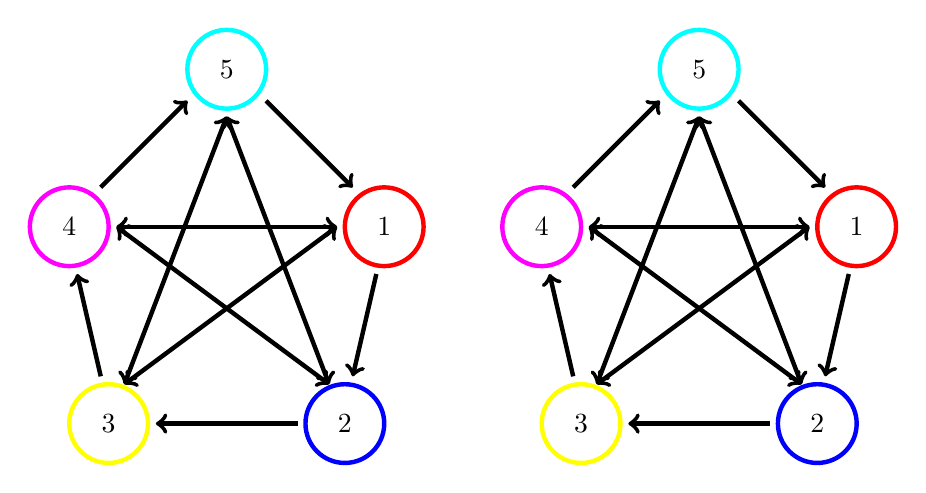
\begin{tikzpicture}
            \definecolor{cl1}{HTML}{FF0000}
            \definecolor{cl2}{HTML}{0000FF}
            \definecolor{cl3}{HTML}{FFFF00}
            \definecolor{cl4}{HTML}{FF00FF}
            \definecolor{cl5}{HTML}{00FFFF}
            \draw[ultra thick, draw=cl1] ( 2.0,2.5) circle (0.5cm) node {$1$};
            \draw[ultra thick, draw=cl2] ( 1.5,0.0) circle (0.5cm) node {$2$};
            \draw[ultra thick, draw=cl3] (-1.5,0.0) circle (0.5cm) node {$3$};
            \draw[ultra thick, draw=cl4] (-2.0,2.5) circle (0.5cm) node {$4$};
            \draw[ultra thick, draw=cl5] ( 0.0,4.5) circle (0.5cm) node {$5$};
            \draw[ultra thick,  ->] ( 1.9,1.9) -- ( 1.6,0.6);
            \draw[ultra thick,  ->] ( 0.9,0.0) -- (-0.9,0.0);
            \draw[ultra thick,  ->] (-1.6,0.6) -- (-1.9,1.9);
            \draw[ultra thick,  ->] (-1.6,3.0) -- (-0.5,4.1);
            \draw[ultra thick,  ->] ( 0.5,4.1) -- ( 1.6,3.0);
            \draw[ultra thick, <->] ( 1.4,2.5) -- (-1.4,2.5);
            \draw[ultra thick, <->] ( 0.0,3.9) -- ( 1.3,0.5);
            \draw[ultra thick, <->] ( 0.0,3.9) -- (-1.3,0.5);
            \draw[ultra thick, <->] (-1.4,2.5) -- ( 1.3,0.5);
            \draw[ultra thick, <->] ( 1.4,2.5) -- (-1.3,0.5);
            \draw[ultra thick, draw=cl1] (8.0,2.5) circle (0.5cm) node {$1$};
            \draw[ultra thick, draw=cl2] (7.5,0.0) circle (0.5cm) node {$2$};
            \draw[ultra thick, draw=cl3] (4.5,0.0) circle (0.5cm) node {$3$};
            \draw[ultra thick, draw=cl4] (4.0,2.5) circle (0.5cm) node {$4$};
            \draw[ultra thick, draw=cl5] (6.0,4.5) circle (0.5cm) node {$5$};
            \draw[ultra thick,  ->] (7.9,1.9) -- ( 7.6,0.6);
            \draw[ultra thick,  ->] (6.9,0.0) -- (5.1,0.0);
            \draw[ultra thick,  ->] (4.4,0.6) -- (4.1,1.9);
            \draw[ultra thick,  ->] (4.4,3.0) -- (5.5,4.1);
            \draw[ultra thick,  ->] (6.5,4.1) -- (7.6,3.0);
            \draw[ultra thick, <->] (7.4,2.5) -- (4.6,2.5);
            \draw[ultra thick, <->] (6.0,3.9) -- (7.3,0.5);
            \draw[ultra thick, <->] (6.0,3.9) -- (4.7,0.5);
            \draw[ultra thick, <->] (4.6,2.5) -- (7.3,0.5);
            \draw[ultra thick, <->] (7.4,2.5) -- (4.7,0.5);
        \end{tikzpicture}
        \caption{\imgtabtitle A}
        \label{fig:rot5}
    \end{figure}